% !TeX root = ../main.tex
\chapter{PROJECT MANAGEMENT PLAN}

\section{Problem Setting}

\subsection{Name of Capstone Project}
\textbf{English:} Integrating Large Language Models (LLM) Into Web-Based Cyber Range for Automated Security Analysis and Training.

\textbf{Vietnamese:} Tích hợp các mô hình ngôn ngữ lớn (LLM) vào Cyber Range dựa trên web để phân tích và đào tạo bảo mật tự động.

\subsection{Problem Abstraction}
At an abstract level, this project addresses a fundamental limitation in current cybersecurity training platforms: the imbalance between infrastructure simulation and analytical skill development. Most existing Cyber Range environments prioritize the deployment of virtual machines, vulnerable services, and attack tools. While these environments successfully replicate technical infrastructures, they often fail to adequately support the cognitive and analytical processes required in real-world Security Operations Centers (SOCs).

\begin{figure}[H]
	\centering
	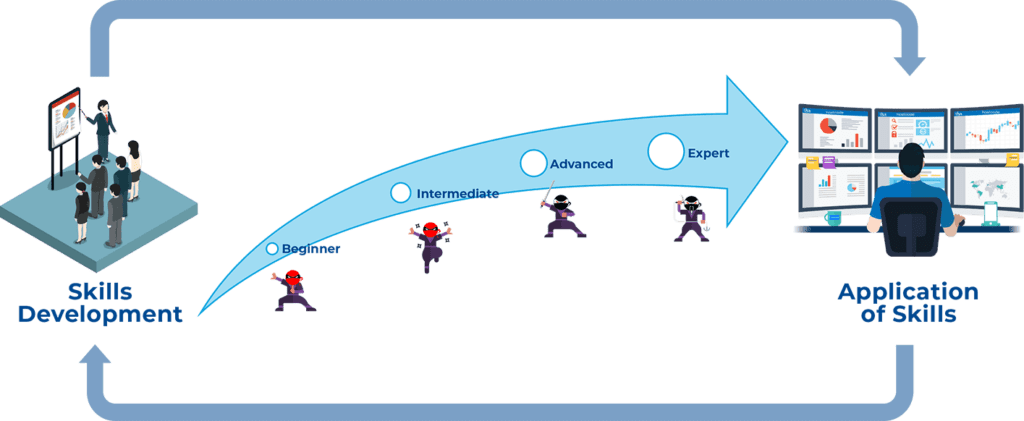
\includegraphics[width=0.95\textwidth]{images/figure 2-1.png}
	\caption{Skill Development to Application of Skills}
\end{figure}

In operational SOC environments, analysts are expected to interpret vast volumes of heterogeneous security data, including web server logs, firewall alerts, intrusion detection events, and system-level audit trails. These data sources are typically fragmented, noisy, and context dependent. Novice analysts frequently struggle to correlate isolated alerts into coherent attack narratives, resulting in delayed responses and superficial understanding.

From an educational perspective, this challenge can be abstracted as the difficulty of transforming raw, low-level security telemetry into structured, explainable knowledge that supports learning and decision-making. The proposed project conceptualizes this problem through a three-layer abstraction model:
\begin{itemize}
	\item \textbf{Security Data Generation Layer:} Simulated attack and defense activities executed within isolated Cyber Range environments.
	\item \textbf{Security Data Aggregation and Correlation Layer:} Centralized logging, Web Application Firewall (WAF), reverse proxy, and SIEM components responsible for collecting and correlating events.
	\item \textbf{Intelligent Assistance Layer:} Large Language Models used to analyze correlated events and provide natural-language explanations, insights, and guidance.
\end{itemize}

\subsection{Project Overview}

\subsubsection{The Current Situation}
In recent years, hands-on, scenario-based cybersecurity training has become an essential requirement for both educational institutions and professional training programs. Despite this shift, many existing training environments continue to exhibit several persistent limitations. First, the volume of logs and alerts generated in simulated attacks often overwhelms learners at the basic level. Second, most platforms offer limited real-time feedback, forcing learners to rely on instructors or post-exercise assessments to understand their mistakes. Finally, the scalability of instructor-led instruction is inherently limited, especially in large classes or self-paced learning settings.

These factors combined reduce training effectiveness and hinder the development of independent analytical skills in learners.

\subsubsection{Boundaries of the Solution}
To address the identified limitations, this project proposes the development of a Web-Based LLM-Augmented Cyber Range. In the proposed architecture, each user is provisioned with an isolated training environment, referred to as a user stack. Each user stack includes a vulnerable web application, a reverse proxy, a Web Application Firewall (WAF), and an attacker machine. All security events generated within these environments are centrally collected and processed by a Security Information and Event Management (SIEM) system.

A Large Language Model is integrated as an intelligent SOC assistant within the platform. Its primary function is to analyze selected security events and alerts, generate human-readable explanations of attack behaviors, and provide context-aware guidance on investigation and mitigation strategies. This approach transforms the Cyber Range from a passive simulation environment into an interactive, guided learning system.

\begin{figure}[H]
	\centering
	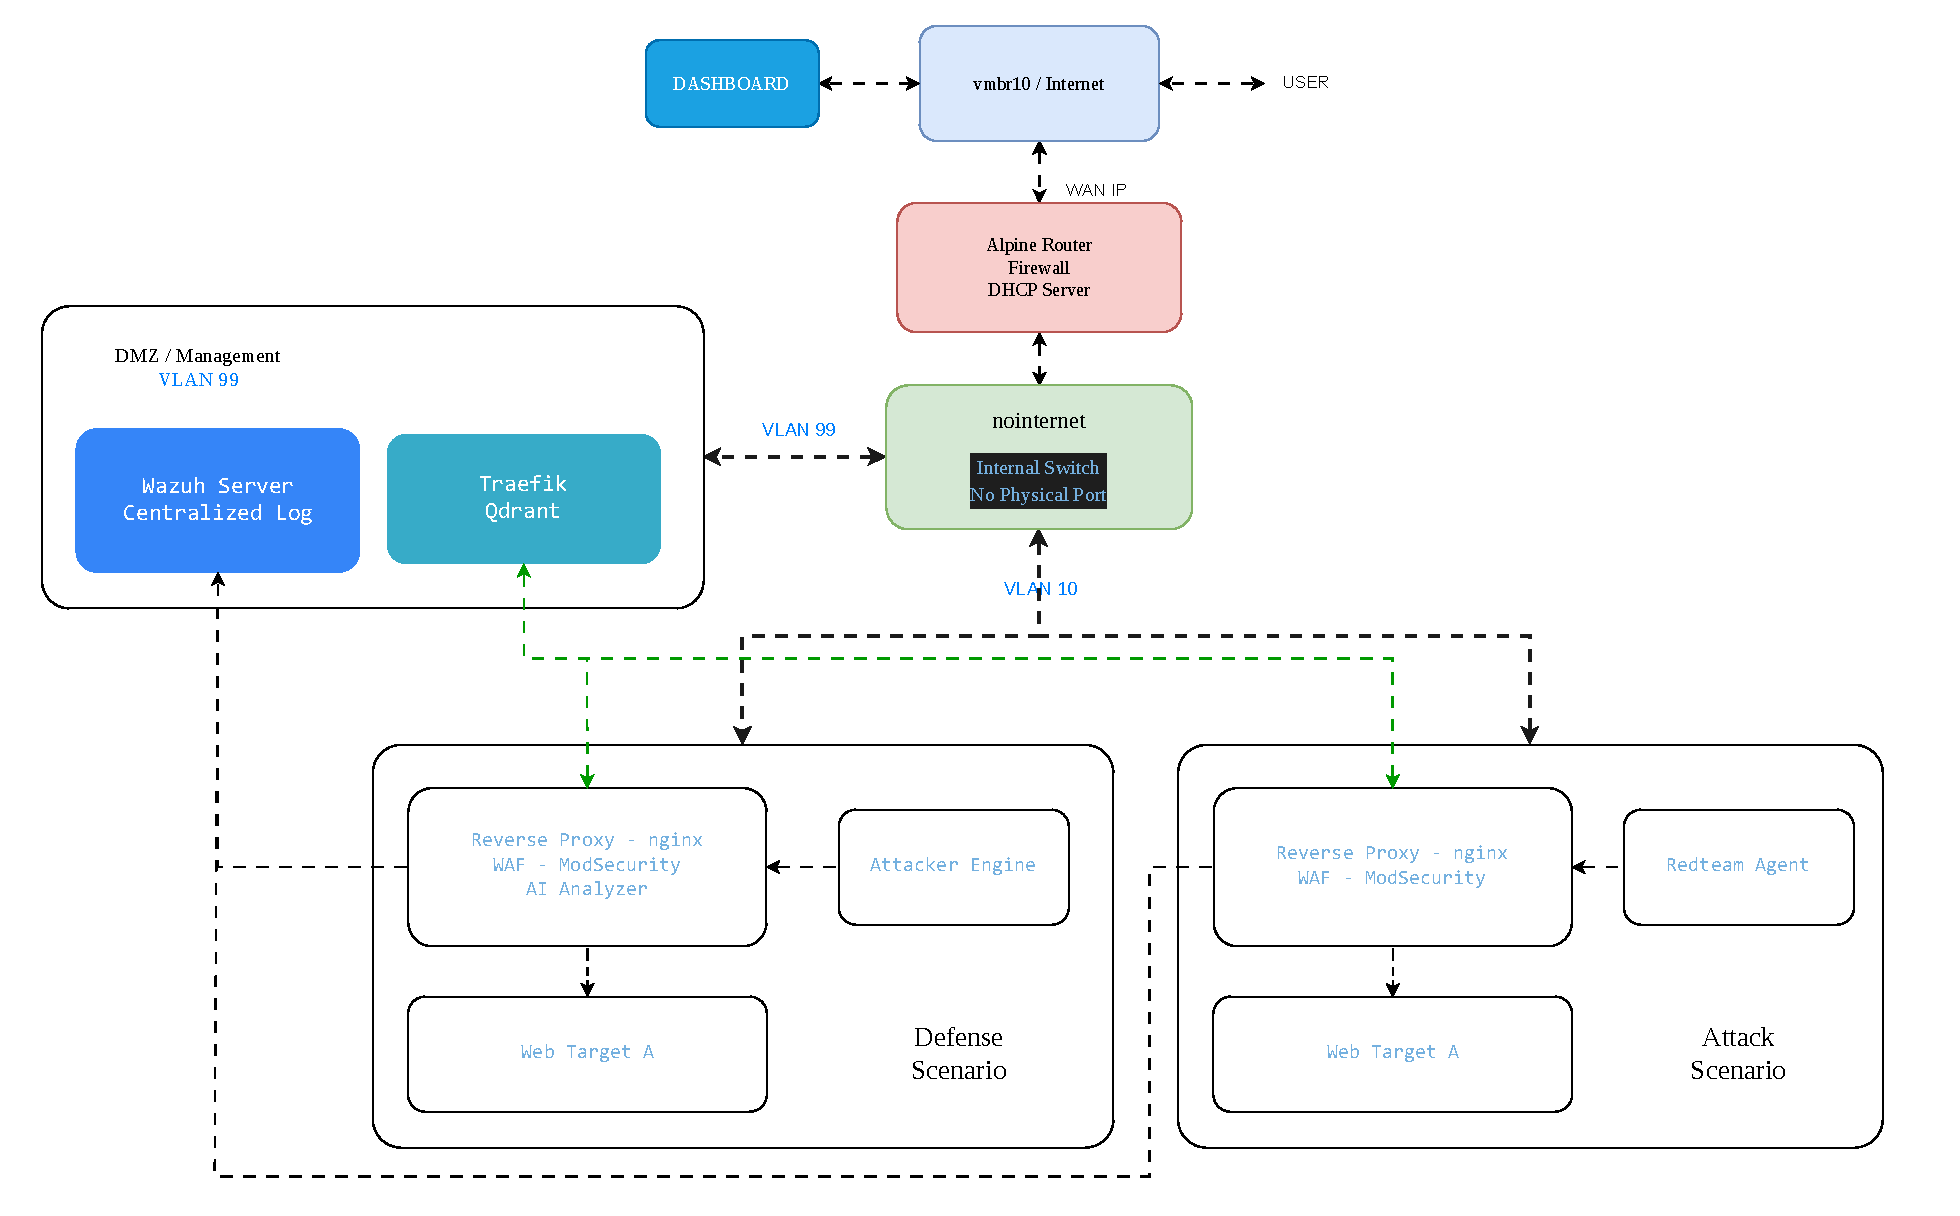
\includegraphics[width=0.95\textwidth]{images/system_flow.pdf}
	\caption{Proposed infrastructure architecture of the cyber range platform.}
	\label{fig:infra-arch}
\end{figure}

\subsubsection{Project Environment}
\begin{table}[H]
	\centering
	\begingroup
	\setlength{\tabcolsep}{3pt}
	\renewcommand{\arraystretch}{1.1}
	\small
	\begin{tabularx}{\textwidth}{|p{0.65cm}|p{2.8cm}|p{0.95cm}|p{0.95cm}|p{1.1cm}|X|p{1.45cm}|}
		\hline
		\textbf{No.} & \textbf{OS} & \textbf{CPU} & \textbf{RAM} & \textbf{Disk} & \textbf{Purpose} & \textbf{Qty.} \\
		\hline
		01 & Alpine Linux & 1 core & 0.5 GB & 4 GB & Router, Firewall, DHCP Server for internal VLAN routing and traffic control & 1 \\
		\hline
		02 & Ubuntu Server 22.04 LTS & 2 cores & 2 GB & 100 GB & Management \& DMZ node hosting Traefik Reverse Proxy, Apache Guacamole, and AI Engine services & 1 \\
		\hline
		03 & Ubuntu Server 22.04 LTS & 10 cores & 8 GB & 60 GB & Centralized SIEM server (Wazuh) for log collection, correlation, and monitoring & 1 \\
		\hline
		04 & Ubuntu Server 22.04 LTS & 4 cores & 6 GB & 30 GB & User training stack including Web Target, nginx Reverse Proxy, WAF (ModSecurity), and attacker machine & 1 per\ user \\
		\hline
		05 & Ubuntu Server 22.04 LTS & 2 cores & 2 GB & 20 GB & Additional internal services for testing, log forwarding, and system integration validation & 1 \\
		\hline
		06 & Proxmox VE Host & 13 cores & 10.5 GB & 74 GB & Virtualization host managing all virtual machines and isolated Cyber Range environments & 1 \\
		\hline
	\end{tabularx}
	\endgroup
	\caption{Development environment}
\end{table}
\FloatBarrier

\section{Project Organization}

\subsection{Solution Process Model}
The project follows an iterative and incremental development model combined with the Scrum framework. This approach was chosen to meet changing requirements, minimize technical risks from the outset, and ensure continuous validation of design decisions. Scrum allows the project team to break down complex development tasks into manageable sprints, each producing verifiable products.

At a high level, the system's operational process unfolds as follows: Users access the platform through a web-based dashboard and connect to their designated environment via Apache Guacamole, providing secure access without the need for client-side software installation. Attack and defense operations are performed in isolated user stacks, generating logs from the WAF, reverse proxy, and host operating system. These logs are aggregated and correlated by the SIEM system. The selected events are then forwarded to the LLM analysis module, which generates contextual interpretations and recommendations for the trainee.

To make implementation and validation more practical, this project also defines explicit end-to-end flow views for each major actor and subsystem. These flow views are used as technical references during development, sprint planning, and test-case design. Instead of treating the architecture only as static blocks, the team models how requests, events, and decisions move between components under normal operation and under attack-driven conditions.

The flow-oriented approach provides the following management and engineering benefits:
\begin{itemize}
\item Clarifies handoff points between infrastructure, backend services, SIEM processing, and AI analysis.
\item Makes debugging easier by identifying where delays, dropped events, or processing errors may occur.
\item Supports role assignment because each teammate can own specific flow segments and validation checkpoints.
\item Improves documentation quality by linking diagrams directly to implementation milestones.
\end{itemize}

\setlength{\LTpre}{0pt}
\setlength{\LTpost}{0pt}
\subsection{Detailed Operational Flows}
This subsection summarizes the primary flow diagrams that guide the implementation and integration process. The diagrams are organized by actor perspective and subsystem perspective so the team can validate both user behavior and platform internals.

\subsubsection{Admin Main Flow}
The admin flow focuses on environment provisioning, policy control, user-stack lifecycle, and monitoring supervision. It is used to verify that administrative operations are auditable, permission-aware, and resilient against configuration mistakes.

\begin{figure}[H]
\centering
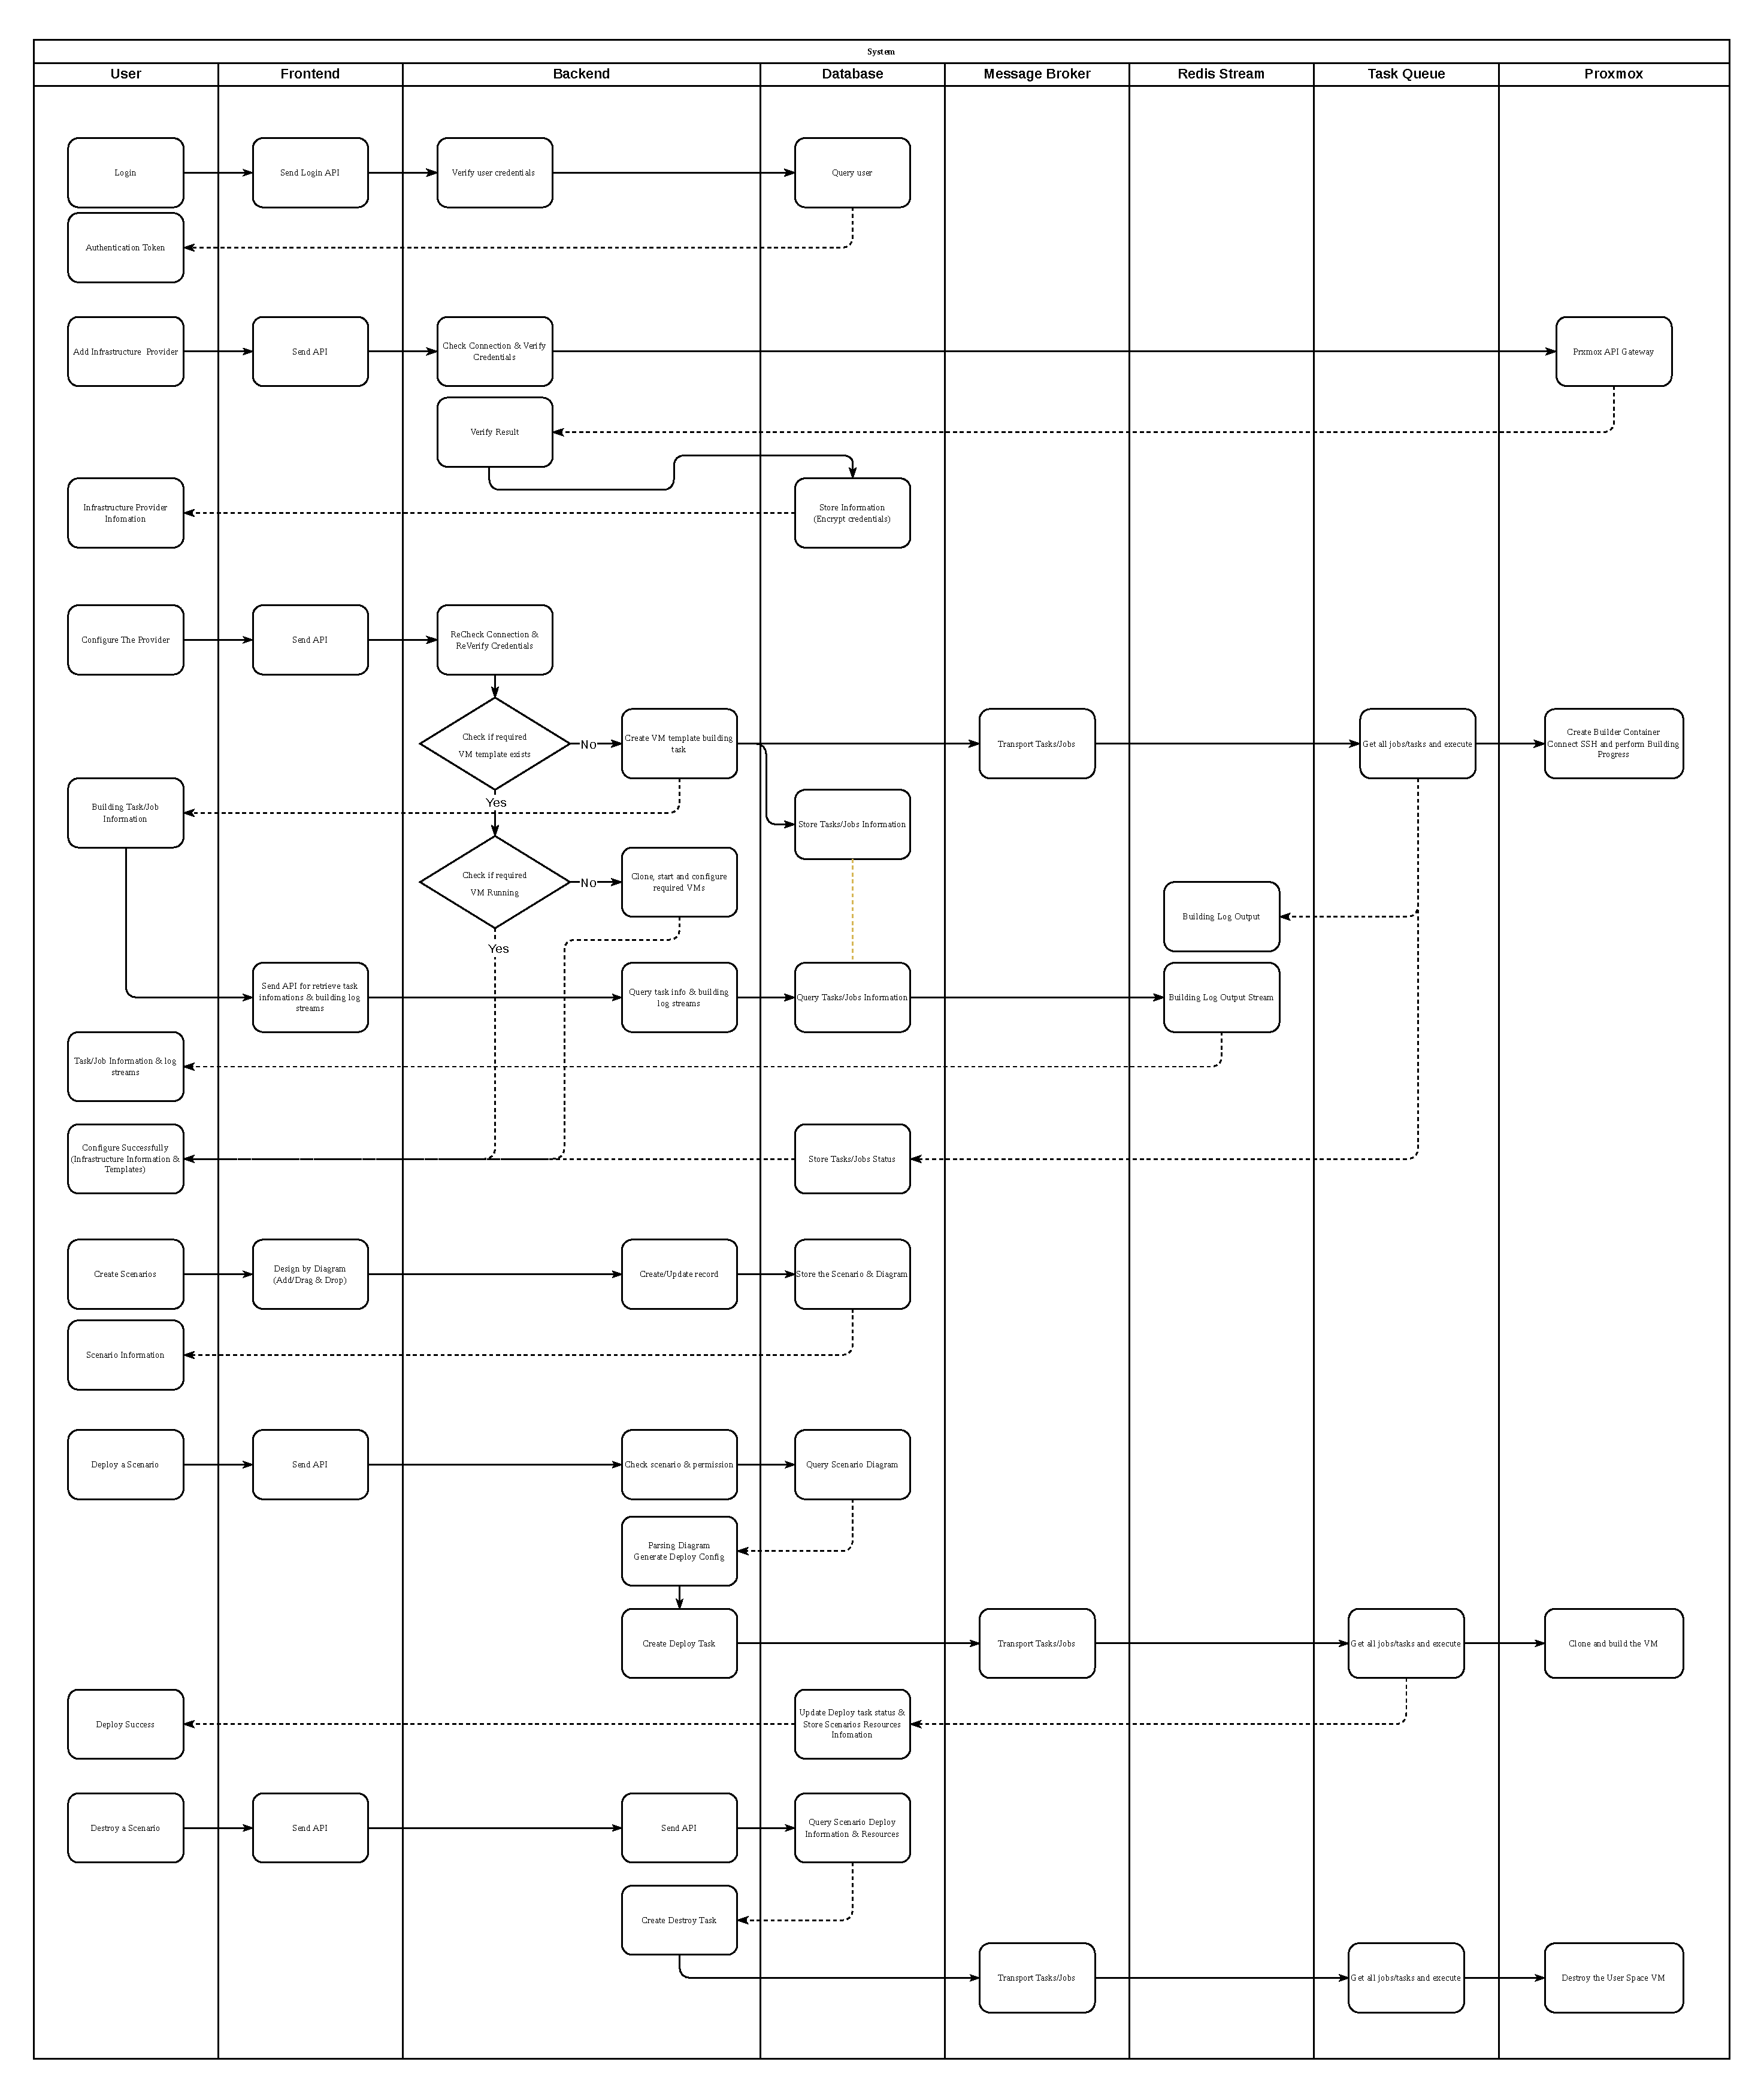
\includegraphics[width=0.95\textwidth]{images/rendered/Admin Main Flow.png}
\caption{Administrative workflow for managing cyber range operations}
\label{fig:admin-main-flow}
\end{figure}

\subsubsection{User Main Flow}
The user flow captures learner actions from login to exercise execution, alert review, and AI-assisted interpretation. This flow ensures that the training journey is coherent, measurable, and aligned with intended learning outcomes.

\begin{figure}[H]
\centering
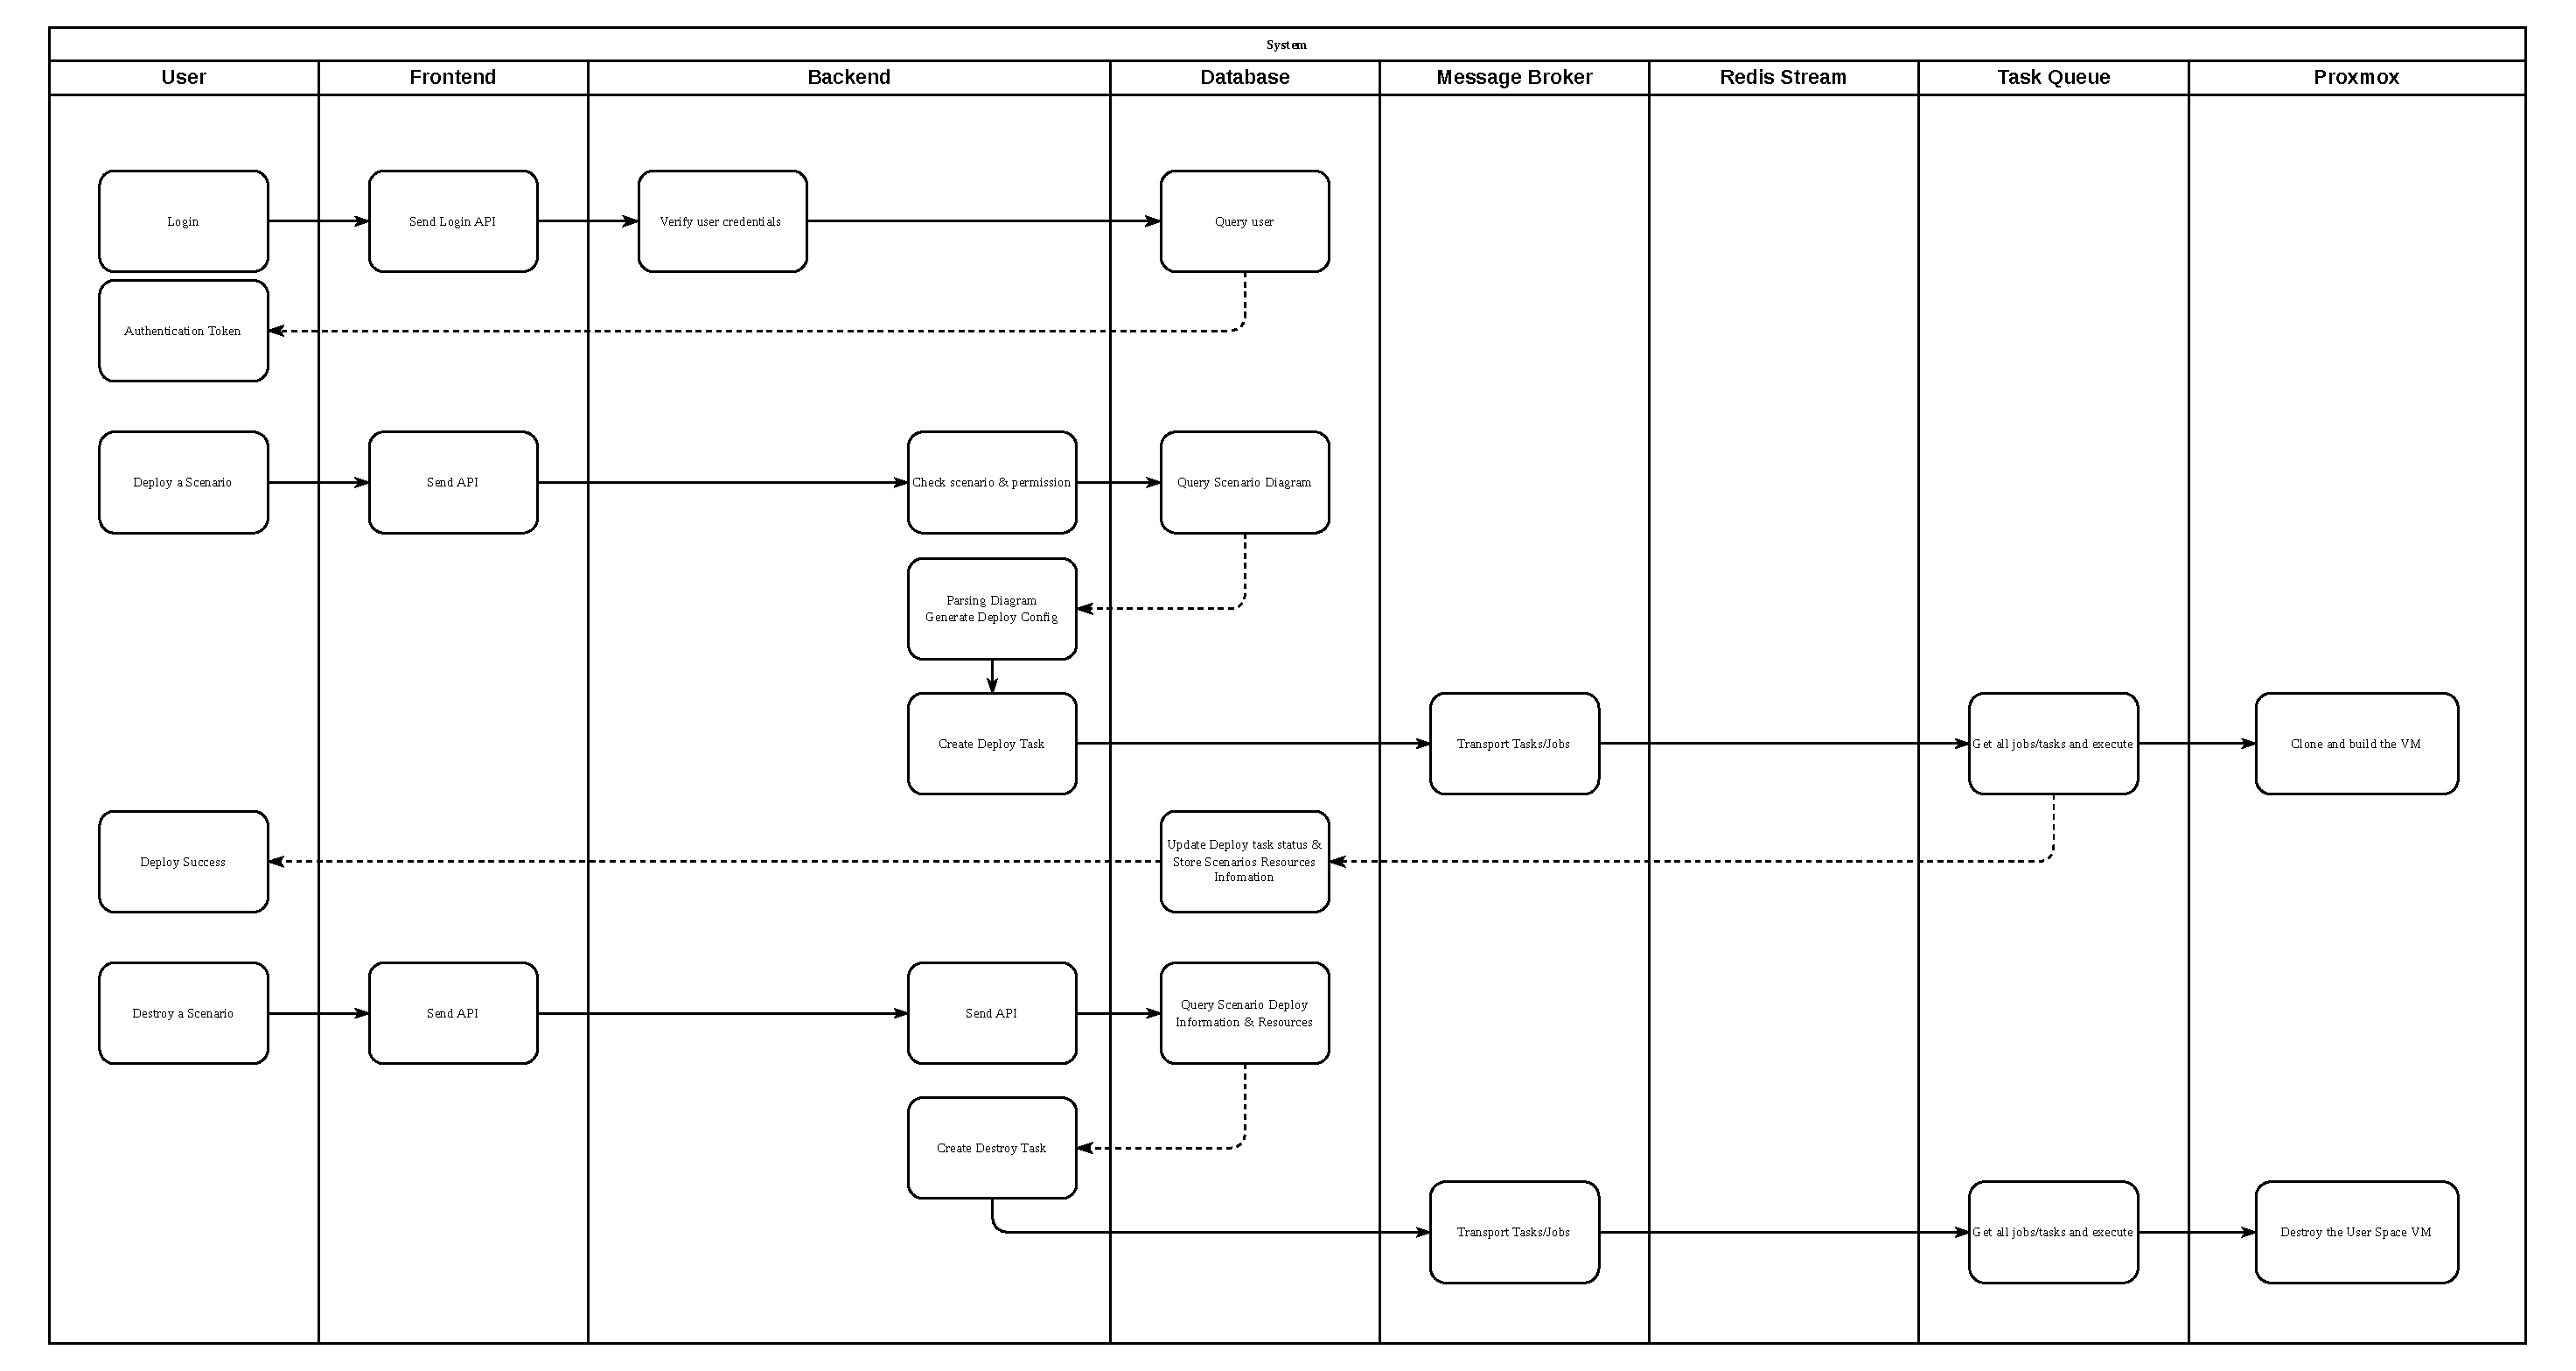
\includegraphics[width=0.95\textwidth]{images/rendered/User Main Flow.png}
\caption{Primary user interaction flow in the cyber range platform}
\label{fig:user-main-flow}
\end{figure}

\subsubsection{User Space Flow}
The user space flow describes how user-initiated actions and HTTP traffic move through the operational components of the platform, from management access to AI-assisted analysis outputs. This view emphasizes the end-to-end data path that links frontend interactions, reverse proxy monitoring, traffic replay, normalization, and service-level analysis.

In this flow, user and admin interactions first reach the management backend, which coordinates control operations and stores configuration state in the management database. Attack or training traffic then passes through the NGINX and ModSecurity layer, where request inspection and security logging are performed before logs are forwarded through Wazuh-related monitoring and HTTP ingest services.

A replay and forwarding stage is used to preserve realistic HTTP traces for backend service processing and AI analysis. The AI analyzer service receives normalized events, generates contextual interpretations, and stores results in the logs database for later review and dashboard presentation.

\begin{figure}[H]
\centering
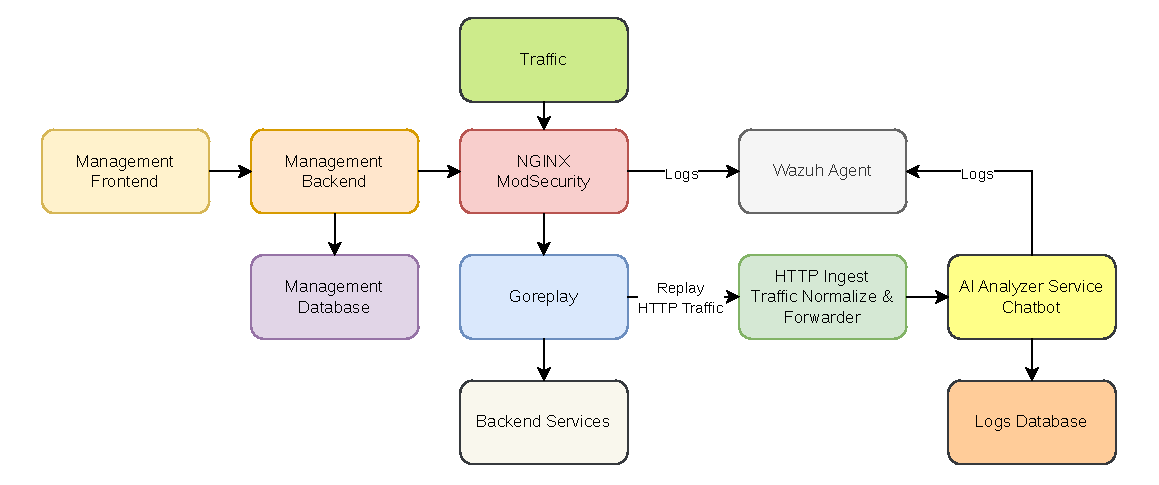
\includegraphics[width=0.95\textwidth]{images/User Space.pdf}
\caption{User space data flow across management, monitoring, and AI analysis}
\label{fig:user-space-flow}
\end{figure}

\subsubsection{User Use Case Flow}
The user use case flow defines the major functional interactions between platform actors and scenario-management capabilities. The diagram shows two primary actors (Admin and User), where the Admin performs full lifecycle operations and the User performs scenario participation and resource access actions.

Core use cases include login, viewing scenarios, accessing resources, and managing scenario execution. Administrative capabilities additionally include scenario design, system settings configuration, infrastructure provider management, user-role management, and controlled teardown of scenario runs.

This use-case perspective complements the system-flow diagrams by clarifying functional permissions, helping the team design role-based access control policies and prioritize feature implementation according to actor responsibility.

\begin{figure}[H]
\centering
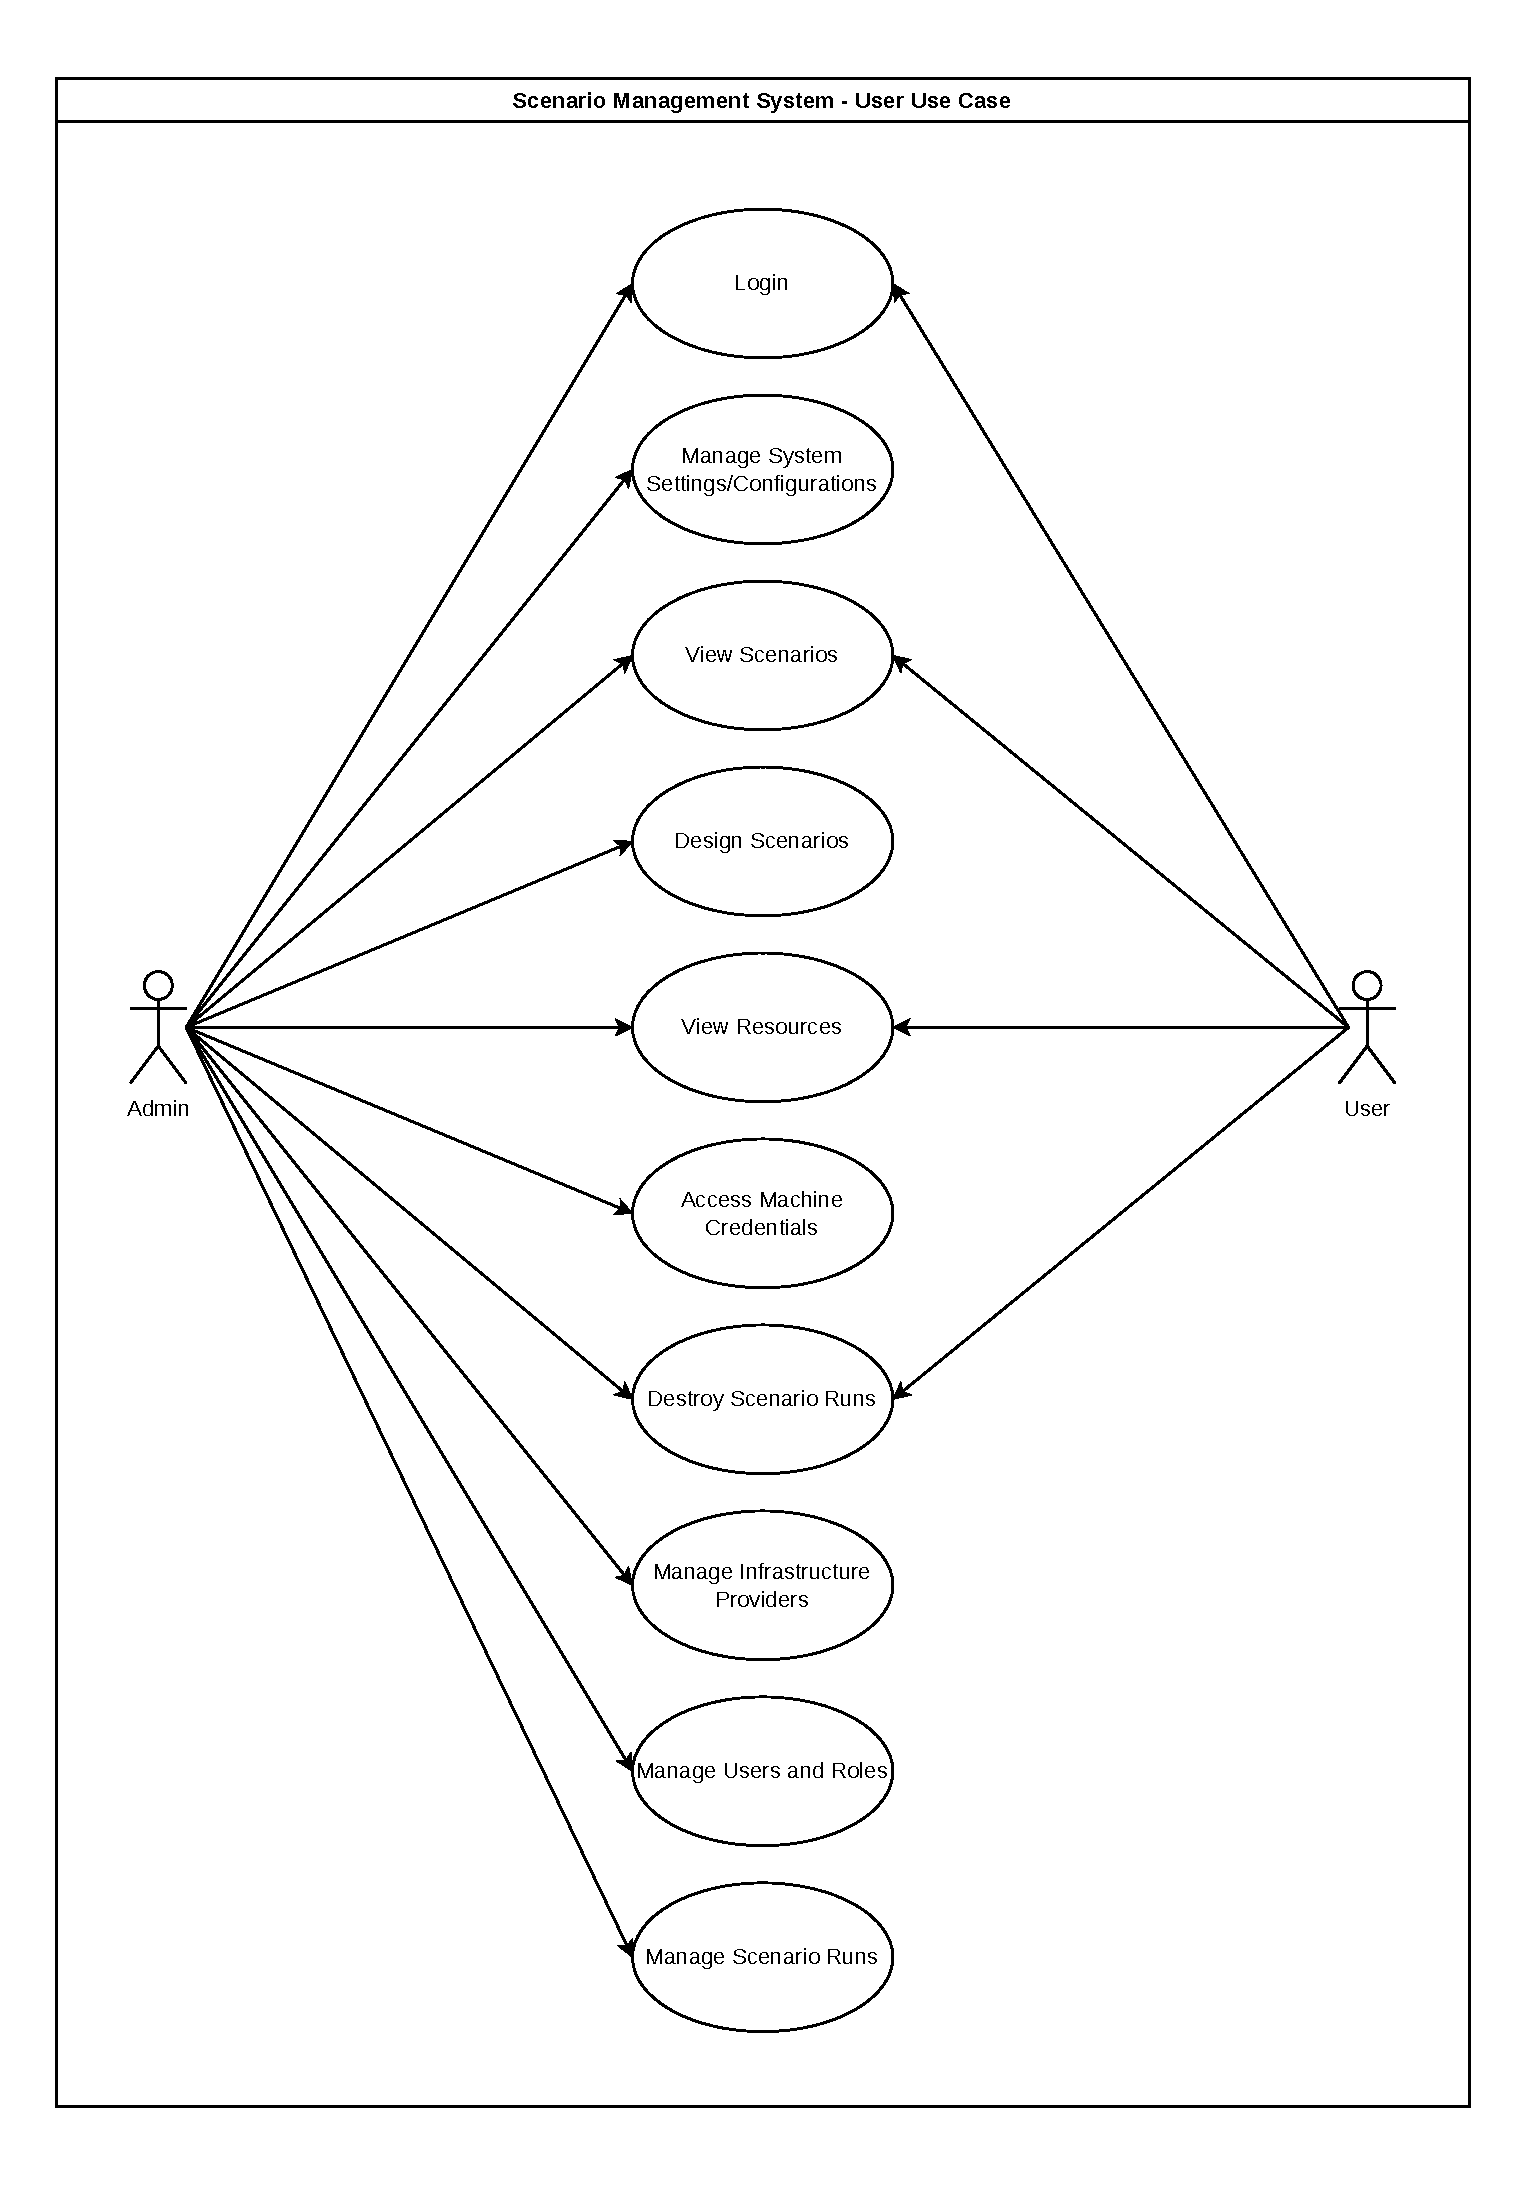
\includegraphics[width=0.95\textwidth]{images/rendered/User Use Case.png}
\caption{User and admin use-case interactions in the scenario management subsystem}
\label{fig:user-use-case-flow}
\end{figure}

\subsubsection{Blue Team Agent Flow}
The Blue Team agent flow describes how logs are ingested, normalized, correlated, and escalated for AI interpretation. This flow is important for validating response latency and consistency of detection outputs.

\begin{figure}[H]
\centering
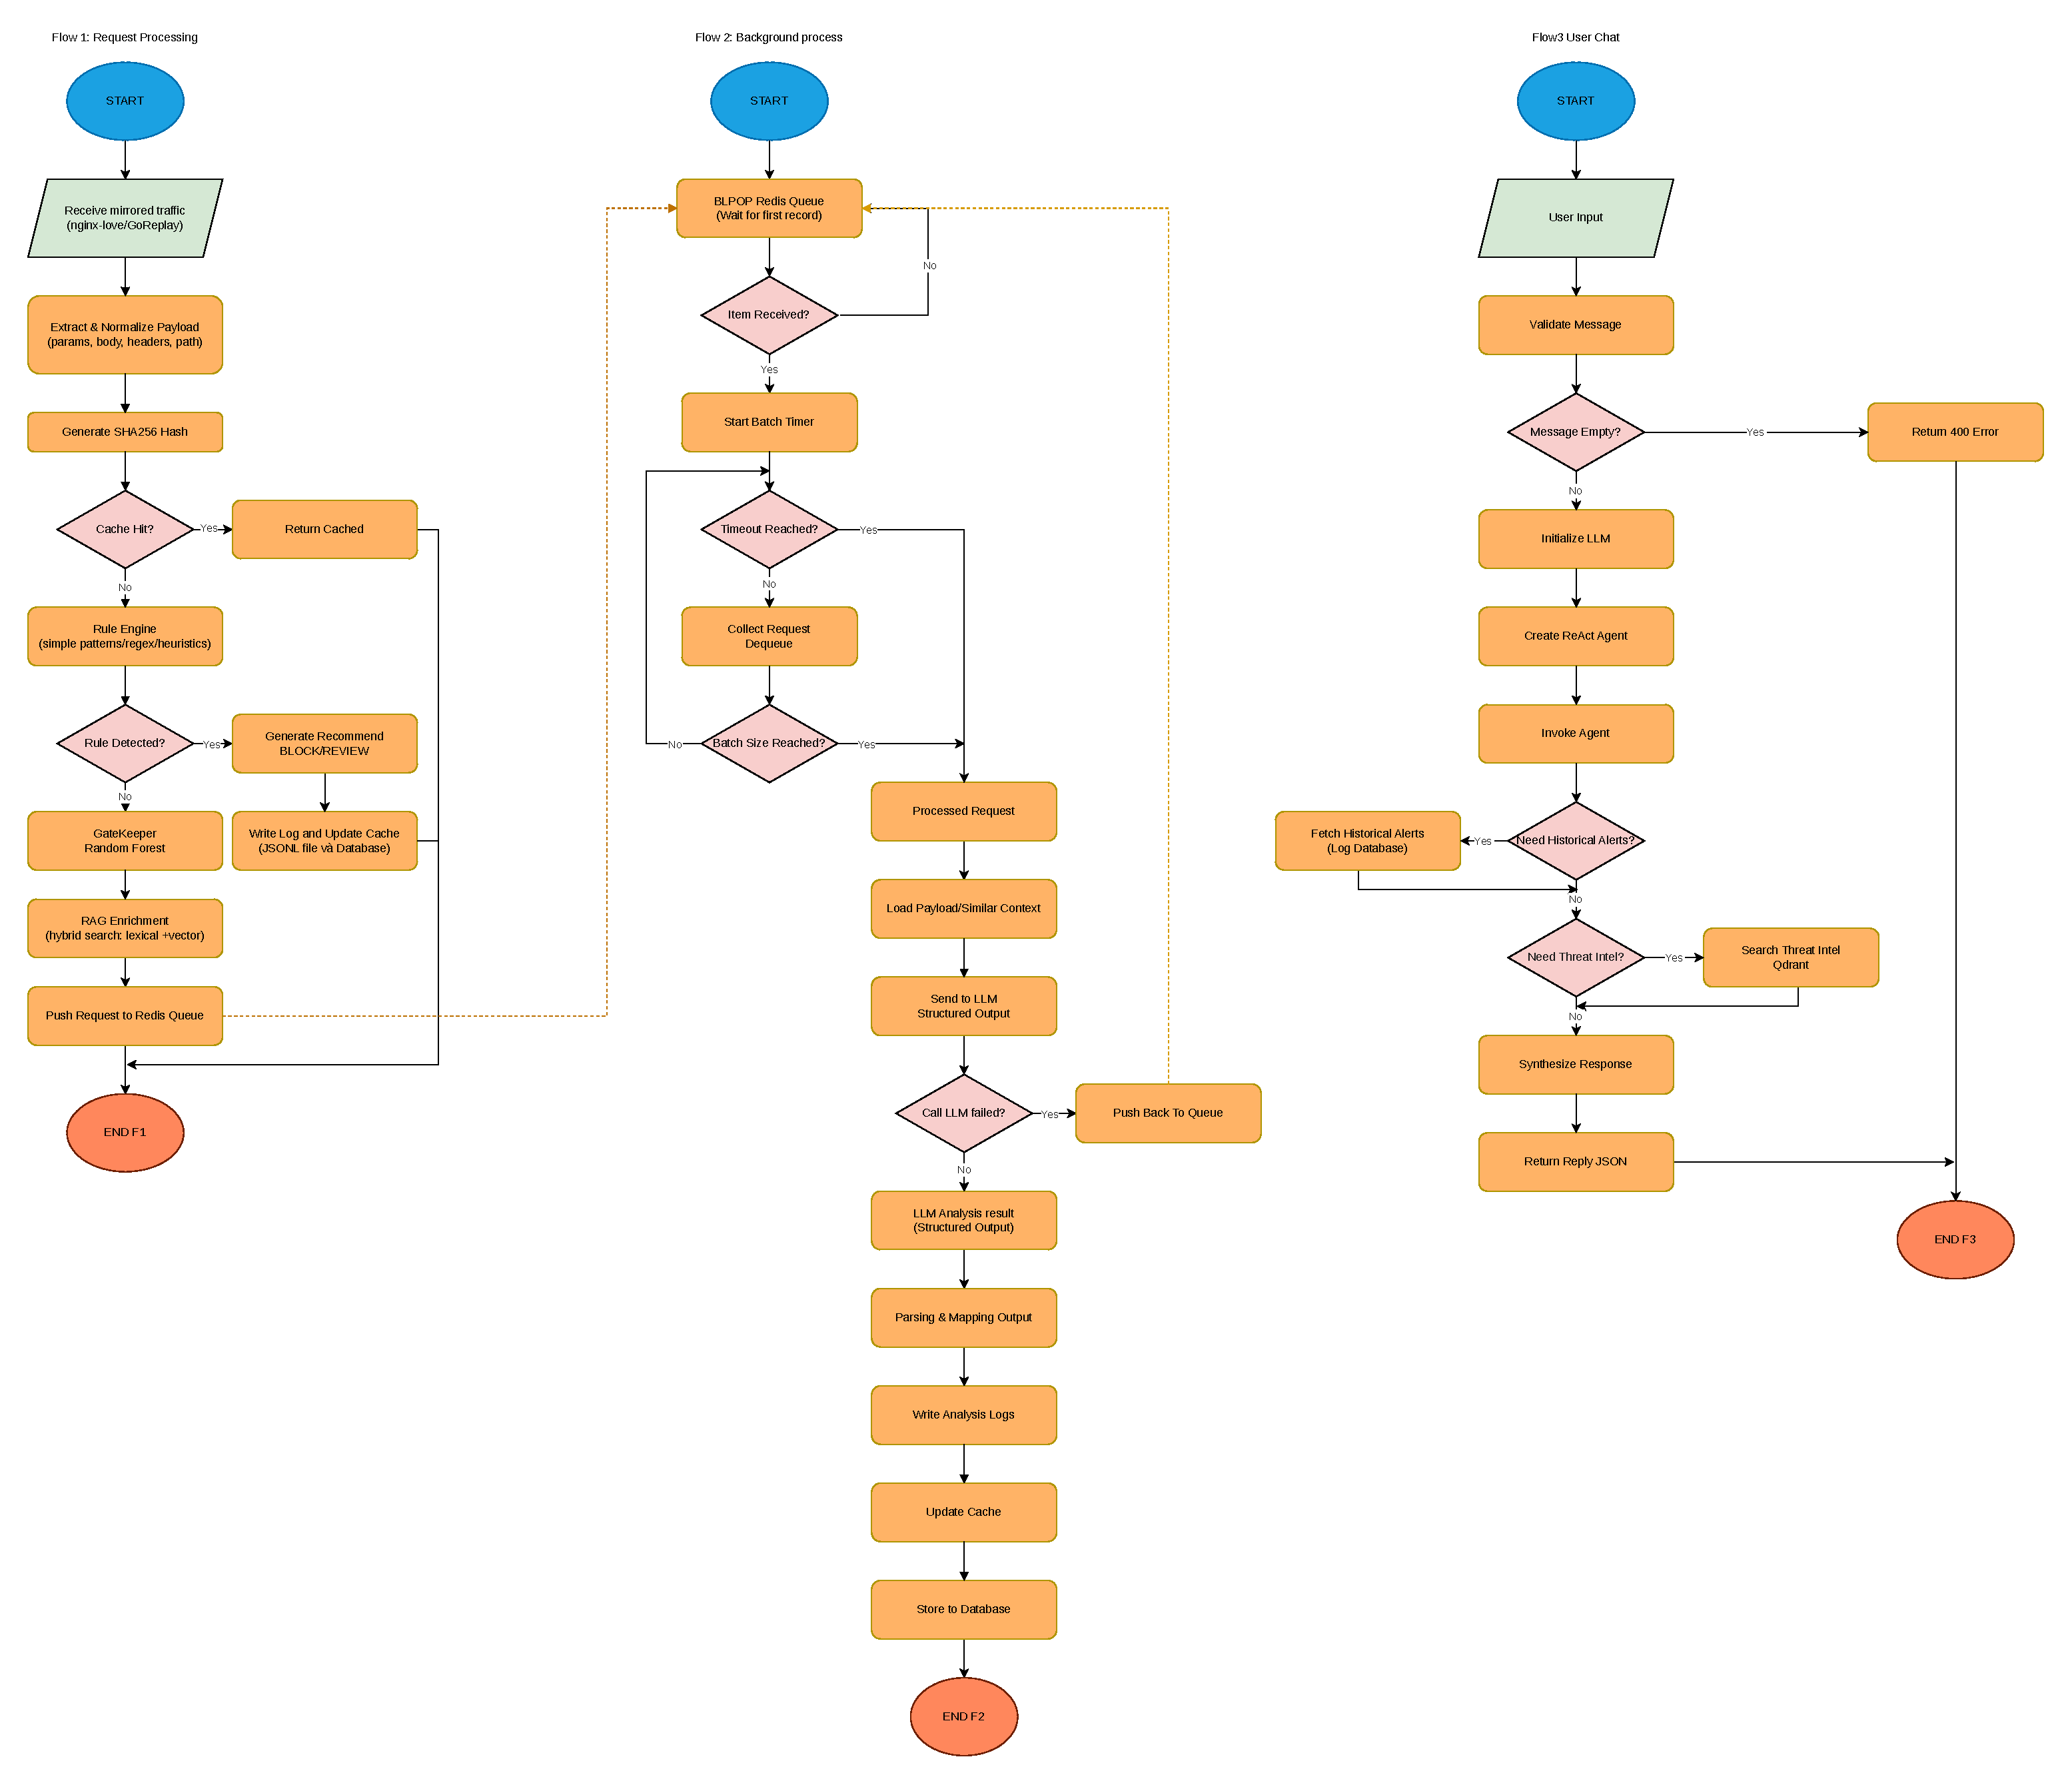
\includegraphics[width=0.95\textwidth]{images/Blueteam_Agent.pdf}
\caption{Blue Team analysis and response pipeline flow}
\label{fig:blueteam-flow}
\end{figure}

\subsubsection{Dashboard Component Flow}
The dashboard component flow explains how frontend modules consume backend endpoints, render alert intelligence, and display AI recommendations. This view is used to coordinate backend contract design and frontend state handling.

\begin{figure}[H]
\centering
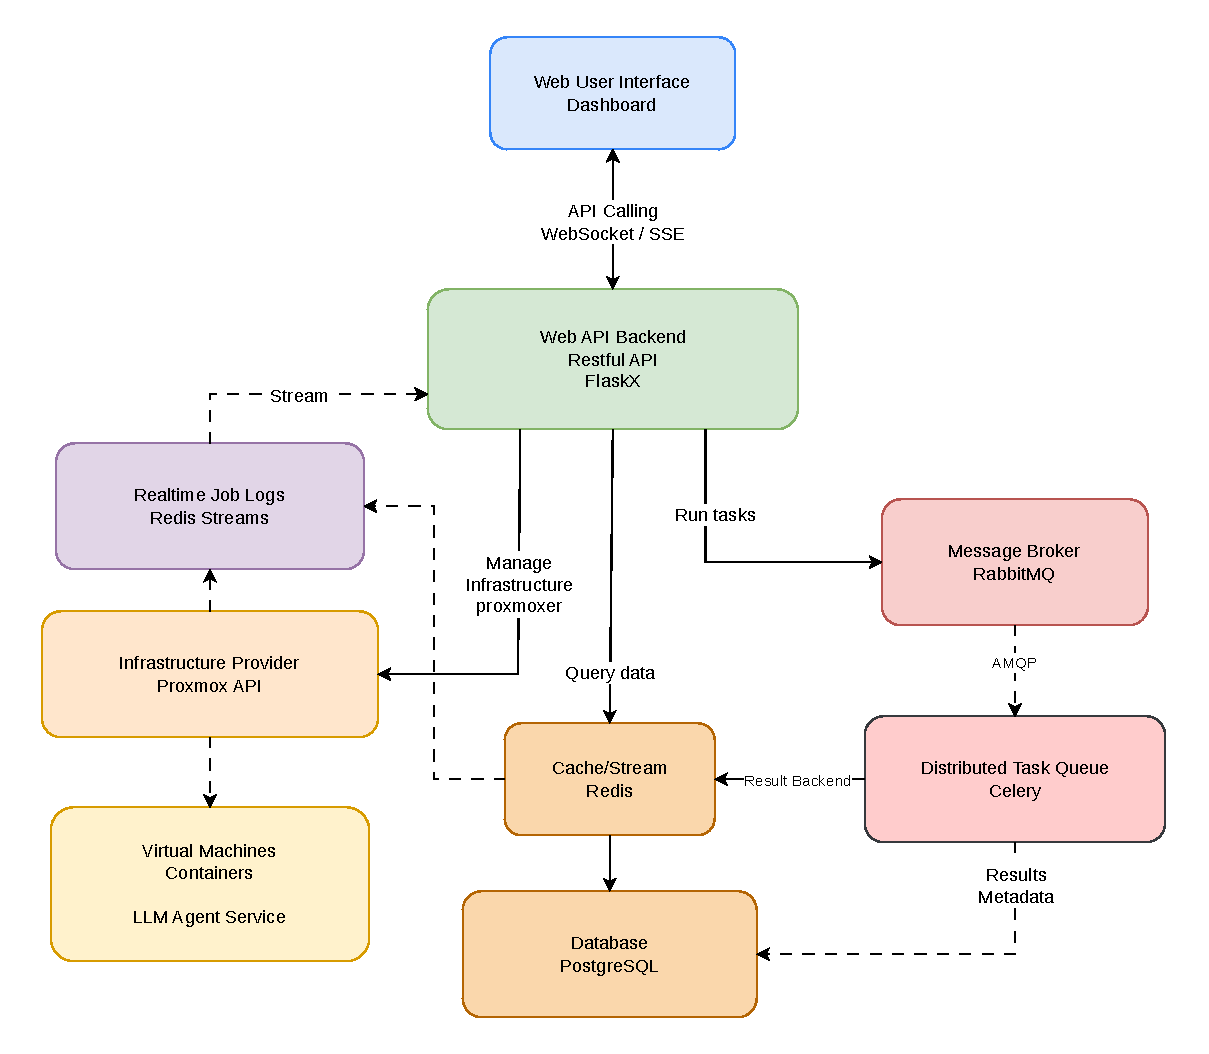
\includegraphics[width=0.95\textwidth]{images/Dashboard.pdf}
\caption{Dashboard component interaction flow for monitoring and analysis}
\label{fig:dashboard-flow}
\end{figure}

\clearpage
\subsection{Roles and Responsibilities}
\begingroup
\setlength{\LTleft}{\fill}
\setlength{\LTright}{\fill}
\setlength{\tabcolsep}{3pt}
\renewcommand{\arraystretch}{1.2}
\small
\begin{longtable}{|p{2.5cm}|p{3.0cm}|p{2.8cm}|p{5.2cm}|}
	\hline
	\textbf{Phase} & \textbf{Full Name} & \textbf{Role} & \textbf{Responsibility} \\
	\hline
	\endfirsthead
	\hline
	\textbf{Phase} & \textbf{Full Name} & \textbf{Role} & \textbf{Responsibility} \\
	\hline
	\endhead

	Initiating & Huỳnh Ngọc Quang & Project Leader & Define project objectives, scope, and overall research direction. Propose the system architecture for the LLM-augmented Cyber Range. Coordinate initial discussions with the supervisor and align technical goals with academic requirements. \\
	\hline
	Initiating & Nguyễn Văn Nhân & Infrastructure Architect & Analyze infrastructure requirements and design the virtualized Cyber Range environment. Define VLAN segmentation, routing strategy, and core services including SIEM, WAF, and reverse proxy. \\
	\hline
	Initiating & Trương Mỹ Vy & AI Researcher & Conduct background research on Large Language Models and their applications in cybersecurity education. Identify feasible LLM use cases for automated security analysis and training assistance. \\
	\hline
	Initiating & Hồ Tài Liên Vy Kha & AI Building and Documentation Coordinator & Conduct initial research on the application of LLMs in cybersecurity training environments. Prepare the initial project proposal, outline report structure, and ensure compliance with capstone documentation standards. \\
	\hline
	Planning & Huỳnh Ngọc Quang & Project Leader & Decompose project objectives into detailed sprint-level tasks and milestones. Define technical deliverables, evaluation criteria, and integration checkpoints. Coordinate planning activities to ensure alignment between infrastructure, AI research, and documentation workstreams. \\
	\hline
	Planning & Nguyễn Văn Nhân & Infrastructure Engineer & Design the detailed infrastructure deployment plan, including Proxmox virtualization layout, VLAN segmentation, routing strategy, and resource allocation. Plan scalability for multi-user Cyber Range environments and ensure isolation between user stacks. \\
	\hline
	Planning & Trương Mỹ Vy & AI Researcher & Design the AI-assisted security analysis workflow, focusing on how security events and logs are transformed into structured inputs for LLM processing. Define research hypotheses related to AI effectiveness in cybersecurity training. \\
	\hline
	Planning & Hồ Tài Liên Vy Kha & AI Building and Documentation Coordinator & Plan the AI implementation architecture using the LangGraph framework for LLM orchestration. Design the AI interaction flow between SIEM outputs and the web-based dashboard. Prepare detailed documentation outlines and reporting templates. \\
	\hline
	Executing & Huỳnh Ngọc Quang & Infrastructure Engineer & Oversee system implementation progress and coordinate integration between infrastructure components, AI services, and the dashboard. Validate intermediate deliverables and ensure adherence to the planned timeline. \\
	\hline
	Executing & Nguyễn Văn Nhân & Infrastructure Engineer & Deploy and configure Cyber Range infrastructure components, including the Alpine-based router, DMZ services, SIEM server, reverse proxies, WAF, and isolated user stacks. Ensure network stability, secure access, and proper log forwarding. \\
	\hline
	Executing & Trương Mỹ Vy & AI Researcher & Conduct experimental evaluation of AI-assisted security analysis. Test different prompt strategies and analyze the quality, accuracy, and usefulness of LLM-generated explanations within training scenarios. \\
	\hline
	Executing & Hồ Tài Liên Vy Kha & AI Building and Documentation Coordinator & Implement AI pipelines using the LangGraph framework to orchestrate LLM workflows. Integrate AI-generated outputs into the web-based user interface. Continuously update technical documentation based on implementation progress. \\
	\hline
	Deployment & Huỳnh Ngọc Quang & Project Leader & Coordinate system deployment and conduct end-to-end integration validation. Prepare demonstration scenarios and training use cases for evaluation and project defense. \\
	\hline
	Deployment & Nguyễn Văn Nhân & Infrastructure Engineer & Optimize system performance, validate VLAN isolation, and ensure secure clientless access through Apache Guacamole. Monitor system stability under simulated user load. \\
	\hline
	Deployment & Trương Mỹ Vy & AI Researcher & Evaluate the effectiveness of AI-assisted analysis in realistic training scenarios. Identify limitations, failure cases, and opportunities for improvement in AI explanations. \\
	\hline
	Deployment & Hồ Tài Liên Vy Kha & AI Building and Documentation Coordinator & Validate the integration between the LangGraph-based AI workflows and the frontend dashboard. Conduct usability testing to ensure AI outputs are clearly presented and understandable for trainees. \\
	\hline
	Closing & Huỳnh Ngọc Quang & Project Leader & Compile the final project report, summarize technical and research outcomes, and coordinate final presentation and defense activities. \\
	\hline
	Closing & Nguyễn Văn Nhân & Infrastructure Engineer & Support final system verification and assisyt in technical explanation during project evaluation and defense. \\
	\hline
	Closing & Trương Mỹ Vy & AI Researcher & Document research findings, experimental results, and identified limitations of AI-assisted security analysis. Propose future research directions, including autonomous AI attacker extensions. \\
	\hline
	Closing & Hồ Tài Liên Vy Kha & AI Building and Documentation Coordinator & Finalize system documentation, AI workflow descriptions (LangGraph-based), and user guides. Ensure consistency between implemented features and academic deliverables. \\
	\hline
	\caption{Team role and responsibilities each phase} \\
\end{longtable}

\subsection{Tools and Techniques}
\renewcommand{\arraystretch}{1.2}
\begin{longtable}{|p{0.7cm}|p{2.8cm}|p{2.8cm}|p{2.0cm}|p{4.7cm}|}
	\hline
	\textbf{No.} & \textbf{Tools} & \textbf{Category} & \textbf{Version} & \textbf{Description} \\
	\hline
	\endfirsthead
	\hline
	\textbf{No.} & \textbf{Tools} & \textbf{Category} & \textbf{Version} & \textbf{Description} \\
	\hline
	\endhead
	01 & Proxmox VE & Virtualization Platform & 8.x & Used as the core virtualization layer to provision, isolate, and manage virtual machines and containers for Cyber Range scenarios. It supports snapshot-based recovery, resource allocation control, and repeatable lab orchestration for multiple users. \\
	\hline
	02 & Ubuntu Server & Operating System & 22.04 LTS & Primary server operating system for SIEM, management, and integration services. Chosen for long-term stability, security patch support, broad package compatibility, and operational reliability in capstone deployment conditions. \\
	\hline
	03 & Alpine Linux & Operating System & 3.x & Lightweight distribution used for router and firewall functions where minimal footprint and reduced attack surface are required. It improves efficiency for network control services such as DHCP, NAT, and segmentation routing. \\
	\hline
	04 & Docker & Containers & 24.x & Provides consistent runtime environments for application and middleware components. Docker simplifies packaging, deployment repeatability, dependency isolation, and rapid rollback when validating attack-defense workflows. \\
	\hline
	05 & Traefik & Reverse Proxy & 2.x & Deployed as an edge ingress layer in the DMZ for traffic routing and service exposure control. It helps centralize request forwarding policies, supports secure entrypoint management, and improves maintainability for multi-service architecture. \\
	\hline
	06 & Nginx & Web Server / Reverse Proxy & 1.24.x & Used in user stacks to proxy traffic to vulnerable applications and to provide logging points for security analysis. Nginx acts as a key telemetry source when combined with ModSecurity and SIEM correlation rules. \\
	\hline
	07 & ModSecurity & Web Application Firewall & 3.x & Provides inspection and filtering for HTTP traffic to detect common web attacks, including SQL Injection and Cross-Site Scripting patterns. It supports rule-driven enforcement and contributes high-value security events to the monitoring pipeline. \\
	\hline
	08 & Wazuh & SIEM Platform & 4.x & Centralized platform for log ingestion, normalization, rule correlation, and alert visualization. Wazuh serves as the SOC analysis backbone and provides the structured event context consumed by AI and dashboard workflows. \\
	\hline
	09 & Apache Guacamole & Remote Access Gateway & 1.5.x & Enables browser-based, clientless access to isolated training machines via protocols such as SSH and RDP. This improves usability for trainees while preserving centralized access control and network boundary protection. \\
	\hline
	10 & LangGraph & LLM Orchestration Framework & 1.0.9 & Implements graph-based orchestration for multi-step AI reasoning. LangGraph is used to model explicit state transitions, tool invocation flow, fallback branches, and response assembly so that security explanations remain structured, traceable, and operationally controllable. \\
	\hline
	11 & Gemini API & LLM Inference API & API-based & Provides the language-model inference layer for natural-language analysis of correlated events. In this project, Gemini-backed workflows are used to generate attack interpretation, investigation hints, and mitigation-oriented explanations suitable for trainee comprehension. \\
	\hline
	12 & FastAPI & API Backend Framework & Latest stable & Serves as the integration backbone connecting SIEM outputs, rule-based preprocessing, retrieval modules, and LangGraph workflows. FastAPI endpoints handle request validation, asynchronous processing, structured responses, and API-level error handling for dashboard consumption. \\
	\hline
	13 & Qdrant & Vector Database & Latest stable & Stores and indexes dense vectors representing security knowledge, historical incidents, and contextual references. Qdrant enables semantic retrieval to enrich AI prompts with relevant context and reduce hallucination risk in generated explanations. \\
	\hline
	14 & HuggingFace Embeddings & Embedding Model Provider & Model-dependent & Converts logs, alerts, and security reference text into vector representations for similarity search. These embeddings support Retrieval-Augmented Generation by supplying targeted context to LLM workflows before response generation. \\
	\hline
	15 & OWASP CRS-style Regex Engine & Rule-based Detection Engine & Custom ruleset & Applies deterministic pattern matching inspired by OWASP Core Rule Set logic to flag known web attack signatures, suspicious payload structures, and anomalous request indicators. It functions as a fast first-pass detection layer before advanced AI analysis. \\
	\hline
	16 & Python & Programming Language & 3.10 & Main implementation language for backend services, orchestration glue code, log preprocessing utilities, evaluation scripts, and automation tasks across the full attack-defense training pipeline. \\
	\hline
	17 & Git & Version Control & Latest & Used for source management, branch-based collaboration, review workflows, and change traceability across infrastructure scripts, backend services, AI workflow definitions, and report artifacts. Git also supports rollback and auditability during iterative sprint delivery. \\
	\hline
	18 & JavaScript & Frontend Development & ES6+ & Used to build interactive dashboard components for lab control, alert visualization, and AI explanation display. JavaScript enables responsive user experience and real-time interaction between trainees and backend services. \\
	\hline
	19 & HTML5 / CSS3 & Frontend Technologies & HTML5 / CSS3 & Provides semantic structure and visual styling for the web interface. These technologies are used to ensure readability, accessibility, and consistent presentation of monitoring and AI-assisted analysis outputs. \\
	\hline
		20 & Custom Training Web Application & Web Application Test Target & Project build & Self-developed web application used to reproduce web attack scenarios such as SQL Injection, XSS, and request manipulation inside the cyber range. This target reflects the project-specific deployment model and provides controlled validation for monitoring and AI-assisted analysis workflows. \\
		\hline
		21 & Custom Containerized Web Stack & Containerized Application Stack & Project build & Containerized web services developed and deployed by the project team to validate scenario orchestration, reverse-proxy inspection, attack logging, and runtime access workflows. This stack is used instead of public training applications so that experiments remain aligned with the designed scenario architecture. \\
		\hline
	\caption{Tools and techniques used in project.} \\
\end{longtable}
\endgroup

\subsection{Retrieval-Augmented Generation for Security Analysis}
Retrieval-Augmented Generation (RAG) is adopted in this project to improve the factual grounding and contextual relevance of AI-generated security explanations. Instead of sending raw alerts directly to the language model, the system first retrieves related knowledge from an indexed security knowledge base and then injects that context into the final prompt. This design is particularly suitable for cyber range training because the same alert may require different interpretations depending on HTTP payloads, WAF signatures, attack stages, and previously observed evidence.

In the proposed platform, the RAG mechanism acts as an intermediate reasoning support layer between SIEM outputs and the Gemini-based analysis module. The retrieval stage reduces ambiguity by attaching semantically relevant references, such as attack descriptions, known payload patterns, rule explanations, and prior incident context, before the response generation step is executed. As a result, the AI assistant is better aligned with the monitored events and less likely to generate vague or hallucinated explanations.

\begin{figure}[H]
	\centering
	
\includegraphics[width=0.9\textwidth]{images/RAG_pic.png}
	\caption{RAG workflow in the proposed platform.}
	\label{fig:rag-workflow}
\end{figure}

The operational logic of the RAG module in this project consists of five main stages. First, structured events are collected from the monitoring pipeline, including WAF alerts, HTTP request traces, rule metadata, and analyst-selected context. Second, these inputs are normalized and converted into a compact query representation suitable for semantic search. Third, the query is embedded and compared against indexed security knowledge stored in Qdrant. Fourth, the most relevant retrieved items are combined with the current alert evidence to form an augmented prompt. Finally, Gemini generates an explanation that is grounded in both observed runtime evidence and retrieved background knowledge.

From an implementation perspective, the RAG workflow complements the LangGraph orchestration layer. LangGraph controls when retrieval is required, how many supporting references should be attached, and how fallback behavior should be handled when the retrieved context is weak or incomplete. This makes the AI pipeline more traceable and more suitable for instructional use, because each answer can be explained as the result of a staged process rather than a single opaque LLM response.

\subsubsection{RAG Processing Logic}
The RAG workflow used in the capstone can be summarized as follows:

\begin{enumerate}
	\item \textbf{Event intake:} Receive selected SIEM alerts, HTTP logs, ModSecurity messages, and user-provided investigation context from the platform.
	\item \textbf{Normalization:} Extract key fields such as request path, parameters, matched rules, suspicious payload fragments, timestamps, and severity level.
	\item \textbf{Query formulation:} Transform the normalized evidence into a concise retrieval query that represents the current security problem.
	\item \textbf{Vector embedding:} Encode the query using the embedding model so that semantic similarity search can be performed.
	\item \textbf{Knowledge retrieval:} Search Qdrant for the top-k most relevant knowledge chunks, including attack descriptions, defensive guidance, and historical references.
	\item \textbf{Context augmentation:} Merge the retrieved knowledge with the original alert evidence to construct a grounded AI prompt.
	\item \textbf{LLM generation:} Submit the augmented prompt to Gemini to produce a human-readable explanation, likely attack interpretation, and suggested response actions.
	\item \textbf{Result presentation:} Return the generated explanation to the dashboard for trainee review and further investigation.
\end{enumerate}

\subsubsection{Algorithmic Description}
The following algorithm summarizes the logical sequence used by the proposed RAG-enabled security assistant.

\noindent\textbf{Algorithm 1: RAG-based security event analysis}

\begin{enumerate}
	\item \textbf{Input:} Correlated security event set $E$, indexed knowledge base $K$, embedding model $M$, vector database $V$, language model $L$.
	\item Parse $E$ to extract the main indicators of compromise, suspicious request features, matched WAF rules, and alert metadata.
	\item Normalize the extracted evidence into a structured analysis object $A$.
	\item Generate a retrieval query $Q$ from $A$.
	\item Encode $Q$ using $M$ to obtain the query vector $q$.
	\item Search $V$ over knowledge base $K$ using $q$ and retrieve the top-k relevant documents $D = \{d_1, d_2, ..., d_k\}$.
	\item Rank or filter $D$ to remove weak or redundant context segments.
	\item Construct an augmented prompt $P$ by combining $A$ with the retained retrieved knowledge.
	\item Submit $P$ to language model $L$ to generate response $R$.
	\item \textbf{Output:} Return $R$ as the final contextual explanation, investigation guidance, and mitigation-oriented suggestion.
\end{enumerate}

This algorithm is intentionally designed for cybersecurity education rather than fully autonomous incident response. The primary goal is not only to classify attacks, but also to explain why an event is suspicious, what evidence supports the interpretation, and what investigation or mitigation steps should be considered next. Therefore, the RAG layer serves both an accuracy function and a pedagogical function inside the web-based cyber range.

\section{Project Management Plan}

\subsection{Tasks}
The project can be divided into several major phases, each further decomposed into a set of minor tasks and distributed across multiple development sprints. Each sprint represents an intensive work cycle aimed at delivering specific outcomes, thereby ensuring steady progress, effective coordination, and continuous validation throughout the project lifecycle.

\subsubsection{Sprint 01: Requirements Analysis and Initial System Design}
During this sprint, the team focuses on gathering, analyzing, and formalizing the project requirements. The objective is to establish a solid conceptual and technical foundation for the LLM-augmented Cyber Range. This sprint emphasizes understanding the attack surface, defining training objectives, and designing the initial system architecture.

The responsibilities in this sprint include the following:
\begin{itemize}
	\item Collecting and documenting functional and non-functional requirements for the Cyber Range platform.
	\item Analyzing the target attack surface and defining the scope of web-based attack and defense scenarios.
	\item Designing the high-level system architecture, including virtualization, network segmentation, SIEM integration, and AI-assisted analysis components.
	\item Selecting core tools and technologies such as Proxmox, Docker, Wazuh, ModSecurity, Apache Guacamole, and the LangGraph framework for LLM orchestration.
	\item Preparing initial architectural diagrams and validating the design with the project supervisor.
\end{itemize}

\subsubsection{Sprint 02: Infrastructure Deployment and Network Configuration}
The second sprint focuses on deploying the foundational infrastructure of the Cyber Range environment. This sprint translates the architectural design into a functional virtualized system capable of supporting isolated training environments.

The responsibilities in this sprint include the following:
\begin{itemize}
	\item Deploying the Proxmox virtualization platform and provisioning virtual machines and containers.
	\item Configuring VLAN-based network segmentation to isolate management, user stacks, and internal services.
	\item Deploying and configuring the Alpine-based router, including firewall rules and DHCP services.
	\item Setting up the DMZ environment and internal switching components.
	\item Configuring secure clientless access using Apache Guacamole.
	\item Verifying network isolation, routing correctness, and controlled internet access.
\end{itemize}

\subsubsection{Sprint 03: Security Services Integration and Log Management}
Sprint 03 focuses on integrating security mechanisms and centralized log management into the Cyber Range. The goal of this sprint is to generate realistic security events and establish a SOC-style monitoring pipeline.

The responsibilities in this sprint include the following:
\begin{itemize}
		\item Deploying self-developed web applications within isolated user stacks to generate controlled attack and monitoring data.
	\item Configuring nginx as a reverse proxy and integrating ModSecurity as a Web Application Firewall.
	\item Executing controlled attack and defense scenarios to generate security logs.
	\item Deploying and configuring the Wazuh SIEM platform for centralized log collection, normalization, and correlation.
	\item Creating alert rules and dashboards to support security monitoring and analysis.
	\item Validating the end-to-end log flow from user stacks to the SIEM system.
\end{itemize}

\subsubsection{Sprint 04: LLM Integration and AI-Assisted Security Analysis}
Sprint 04 is dedicated to integrating artificial intelligence into the Cyber Range. This sprint introduces LLM-based analysis to transform raw security data into contextual, human-readable insights for training purposes.

The responsibilities in this sprint include the following:
\begin{itemize}
	\item Designing AI workflows using the LangGraph framework to orchestrate Large Language Model interactions.
	\item Defining structured inputs for AI analysis based on SIEM alerts, HTTP requests, and correlated security events.
	\item Implementing retrieval-augmented prompting so AI explanations remain grounded in relevant security knowledge.
	\item Integrating AI-generated outputs into the BlueAgent WAF Console and related web-based dashboard views.
	\item Evaluating the accuracy, relevance, and usefulness of AI-assisted explanations in training scenarios.
	\item Refining AI interaction logic based on experimental feedback.
\end{itemize}

\subsubsection{Sprint 05: System Validation, Evaluation, and Documentation}
The final sprint focuses on validating the complete system, evaluating its effectiveness, and finalizing project documentation. This sprint ensures that all components operate cohesively and that project outcomes are clearly documented.

The responsibilities in this sprint include the following:
\begin{itemize}
	\item Conducting end-to-end system testing across infrastructure, security services, AI modules, and the user interface.
	\item Evaluating system performance, stability, and usability under simulated training conditions.
	\item Assessing the effectiveness of AI-assisted analysis in supporting cybersecurity training.
	\item Finalizing technical documentation, system descriptions, and experimental results.
	\item Documenting system limitations and proposing future enhancements, including autonomous AI-driven attacker modules.
	\item Preparing the final report and materials for project presentation and defense.
\end{itemize}

\subsection{Task Sheet: Assignments and Timetable}
\begingroup
\setlength{\LTleft}{\fill}
\setlength{\LTright}{\fill}
\setlength{\tabcolsep}{3pt}
\renewcommand{\arraystretch}{1.1}
\small
\begin{longtable}{|p{3.0cm}|p{2.4cm}|p{1.9cm}|p{1.6cm}|p{4.4cm}|}
	\hline
	\textbf{Task} & \textbf{Assigned To} & \textbf{Estimated Duration} & \textbf{Deadline} & \textbf{Description} \\
	\hline
	\endfirsthead
	\hline
	\textbf{Task} & \textbf{Assigned To} & \textbf{Estimated Duration} & \textbf{Deadline} & \textbf{Description} \\
	\hline
	\endhead
	\hline
	\multicolumn{5}{r}{\textit{Continued on next page}} \\
	\endfoot
	\endlastfoot
	Project planning and scope definition & Huỳnh Ngọc Quang & 1 week & Week 1 & Define project objectives, scope, deliverables, and success criteria for the CyberRange system. \\
	\hline
	CyberRange environment setup & Nguyễn Văn Nhân & 2 weeks & Weeks 2 & Deploy isolated CyberRange stacks including vulnerable web applications and supporting services. \\
	\hline
	Research on web attack patterns & Trương Mỹ Vy & 1 week & Weeks 2 & Study common web attacks (SQLi, XSS, LFI, SSRF, etc.) and their characteristics in HTTP logs. \\
	\hline
	AI preprocessing module development & Hồ Tài Liên Vy Kha & 2 weeks & Week 2 & Implement multi-layer preprocessing logic to classify attacks and reduce LLM invocation. \\
	\hline
	System architecture design & Huỳnh Ngọc Quang & 1 week & Week 3 & Design the overall CyberRange architecture, including attacker, defender, WAF, SIEM, Dashboard and AI workflow components. \\
	\hline
	WAF and reverse proxy configuration & Nguyễn Văn Nhân & 1 week & Week 3 & Configure ModSecurity and reverse proxy to inspect and filter incoming HTTP traffic. \\
	\hline
	AI detection methodology design & Trương Mỹ Vy & 1 week & Week 3 & Propose AI-based detection approaches combining rule-based, heuristic, and LLM-assisted analysis. \\
	\hline
	LLM integration and workflow implementation & Hồ Tài Liên Vy Kha & 1 week & Week 3 & Integrate LLM into the analysis pipeline for handling uncertain or complex attack cases. \\
	\hline
	Risk management and progress tracking & Huỳnh Ngọc Quang & Continuous & Project-wide & Identify project risks, track progress, and adjust plans to ensure project stability. \\
	\hline
	Attack simulation environment & Nguyễn Văn Nhân & 1 week & Week 4 & Set up attacker machines and tools to generate realistic attack traffic for testing. \\
	\hline
	Attack-Defense evaluation metrics & Trương Mỹ Vy & 1 week & Week 5 & Define metrics to measure success of AI attacks versus AI defenses. \\
	\hline
	Attack-Defense feedback loop & Hồ Tài Liên Vy Kha & 1 week & Week 6 & Integrate attack results as feedback to refine defensive AI rules and logic. \\
	\hline
	Final integration review and validation & Huỳnh Ngọc Quang & 1 week & Week 7 & Validate system integration, ensure all components work cohesively, and prepare for final defense. \\
	\hline
	Infrastructure optimization and stability testing & Nguyễn Văn Nhân & 1 week & Week 8 & Optimize performance, ensure isolation between users, and maintain system stability. \\
	\hline
	AI workflow improvement suggestions & Trương Mỹ Vy & Continuous & Project-wide & Propose improvements to reduce unnecessary LLM usage while maintaining accuracy. \\
	\hline
	Documentation of attack scenarios & Hồ Tài Liên Vy Kha & Continuous & Project-wide & Document attack strategies, payloads, and evaluation results in the final report. \\
	\hline
	\caption{Assignment task sheet} \\
\end{longtable}
\endgroup

\subsection{Meeting Minutes}
\begin{table}[!htbp]
	\centering
	\begingroup
	\small
	\setlength{\tabcolsep}{4pt}
	\renewcommand{\arraystretch}{1.1}
	\begin{tabularx}{\textwidth}{|p{3.2cm}|X|}
		\hline
		\textbf{Subject} & SP26IA01 \\
		\hline
		\textbf{Instructor} & Mr. Mai Hoàng Đỉnh \\
		\hline
		\textbf{Location} & FPT HCM Campus\\
		\hline
		\textbf{Attendees} & Huỳnh Ngọc Quang (SE181838), Nguyễn Văn Nhân (SE183547), Trương Mỹ Vy (SE184728), Hồ Tài Liên Vy Kha (SE173290) \\
		\hline
		\textbf{Absence} &  \\
		\hline
		\textbf{Date} & 01/2026 -- 4/2026 \\
		\hline
		\textbf{Time} & 09:30 A.M -- 11:30 A.M every Monday \\
		\hline
	\end{tabularx}
	\caption{Meeting minute}
	\endgroup
\end{table}